\chapter{FTSP+} \label{cap:cap4}
\outlineon=1

\outline{Intro}

\outline{
  \begin{itemize}
    \item Explicar a t�cnica.
    \item Inserir ilustra��o do processo de sincroniza��o com o rel�gio externo. 
    \item Pseudo c�digo
    \item FTSP+ e subsection
  \end{itemize}
}

\section{T�cnica}

\outline{Descrever o processo de c�lculo do tempo de acesso ao meio, e onde foi baseado.}


\section{Modifica��o}

\outline{
   Pseudo c�digo com explica��o do passo-a-passo do algoritmo (no sender e no receiver).
}


In any distributed time synchronization technique, nodes have to tell each other their local time.
Figure \ref{fig:diagrama} depicts this scenario.
The sending node stores its local time $t1'$ in the synchronization message at time $t1$ and orders the message to be sent.
Due to medium random access uncertainties, the sending node only gets access to the medium at time $t2$ and starts sending me message.
$t2-t1$ is called \textit{medium access time}.
The message propagates over the medium for an interval of time $tp$ until it reaches the receiver radio at time $t3$.
$tp$ is the \textit{propagation time}.
Due to interrupt handling policies and packet header processing, the receiver node timestamps the message receipt at time $t4$ with its local time $t4''$.
$t4-t3$ is the \textit{processing time}.

Synchronization inaccuracy happens because the receiving node thinks that at time $t4$ the sender has time $t1'$ and the receiver has time $t4''$.
We can see in Figure \ref{fig:diagrama} that this is not true.
At time $t4$, the sending node has time $t4' = t1' + \mbox{\textit{medium access time}} + \mbox{\textit{propagation time}} + \mbox{\textit{processing time}}$.
MAC layer time-stamping makes \textit{medium access time} and \textit{processing time} equal zero.
Since \textit{propagation time} is negligible ($\sim 1\mu{s}$) \cite{maroti2004}, some synchronization policies --- including FTSP --- can achieve very good accuracy.
However, without MAC layer time-stamping, these times are non-negligible and have to be calculated.

\begin{figure}[htbp]
	\centering
		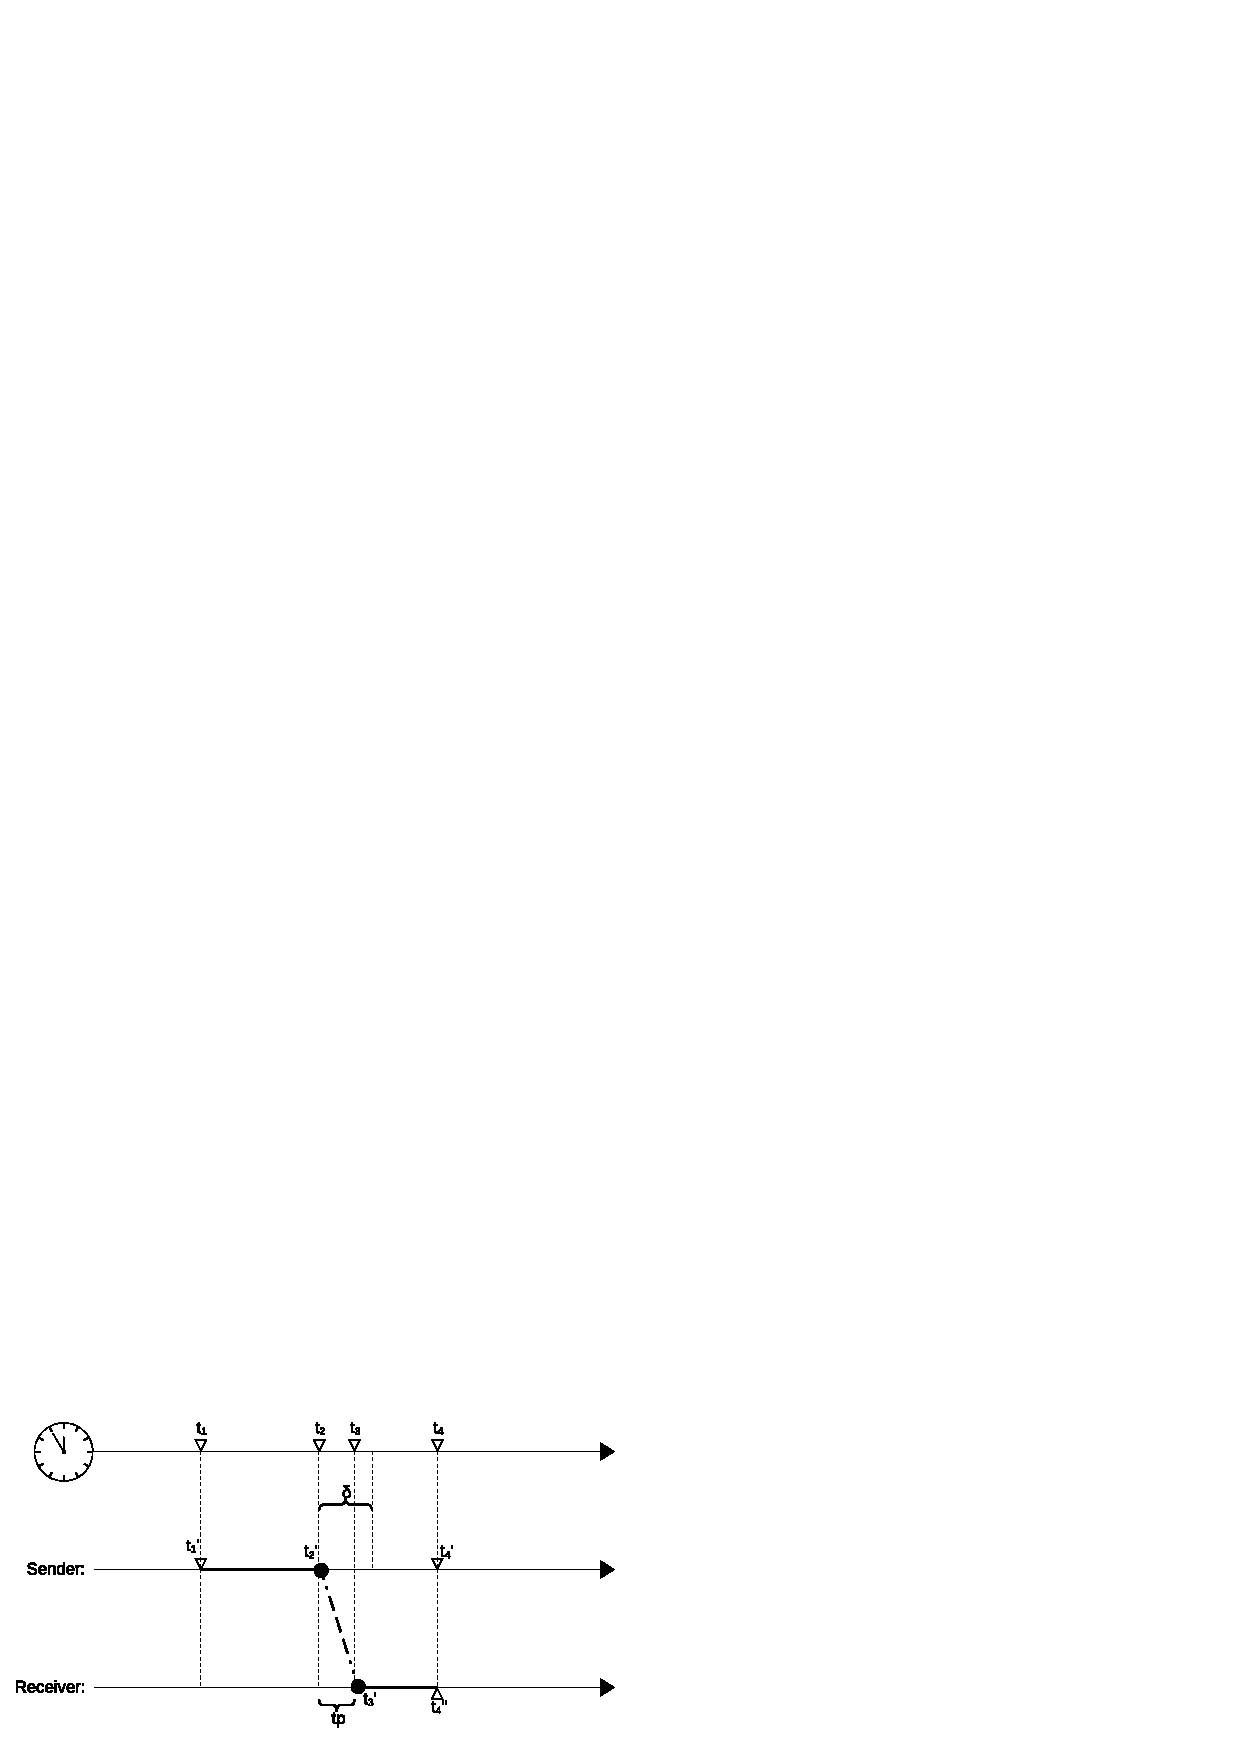
\includegraphics[width=\linewidth]{figuras/diagrama.jpg}
	\caption{Syncronization steps.}
	\label{fig:diagrama}
\end{figure}

FTSP+ calculates \textit{medium access time} using an interrupt handler to time stamp the moment that the node gets medium access to send the synchronization message.
Although medium access is granted at time $t2'$, \textit{medium access timestamp} equals $t2'+\delta$, where $\delta$ is the overhead to process the interrupt handler.

The sender sends a correction message with content $t2'+\delta-t1'$ so the receiver can estimate $t4'$.
Let us call this estimation $\bar{t4'}$.
The receiver calculates $\bar{t4'}$ as in Equation \eqref{eq:estimated_t4}.

\begin{eqnarray}
\bar{t4'} & = & t1' - (t2' + \delta - t1') \nonumber\\
\label{eq:estimated_t4}
\bar{t4'} & = & t1' + \mbox{\textit{medium access time}} + \delta
\end{eqnarray}

The difference between $t4'$ and $\bar{t4'}$, which is the estimation error, is:
\begin{equation}
\label{eq:estimation_error}
t4' - \bar{t4'} = \mbox{\textit{propagation time}} + \mbox{\textit{processing time}} - \delta
\end{equation}

Since \textit{processing time} and $\delta$ are interrupt handler processing latencies, they tend to cancel out each other.
We investigate their values in our experiments in Section \ref{sec:evaluation}.
Remember that \textit{propagation time} is negligible.


\begin{figure}
\begin{Verbatim}[numbers=left,numbersep=1pt,frame=single]
event Radio.receiveSyncMsg(SyncMsg *msg){
  if( msg->rootID < myRootID )
      myRootID = msg->rootID;
  else if( msg->rootID > myRootID
    || msg->seqNum <= highestSeqNum )
      return;
  highestSeqNum = msg->seqNum;
  if( myRootID < myID )
      heartBeats = 0;
  if( numEntries >= NUMENTRIES_LIMIT
    && getError(msg) > TIME_ERROR_LIMIT )
      clearRegressionTable();
  else if (MAC_Time==false){
      addToWaitCorrectionMsgList(msg);
  }else{
      addEntryAndEstimateDrift(msg); 
  }  
}

event Radio.receiveCorrectionMsg(
                            CorrectionMsg *msg){
  applyCorrection(msg);
  addEntryAndEstimateDrift(msg);
}
\end{Verbatim}
 \caption{Receiver algorithm}\vspace{1em}
 \label{fig:receiver_ftspplus}
\end{figure}


As can be seen in Figure \ref{fig:receiver_ftspplus}, an FTSP+ receiver has routines to handle two different types of income messages: \texttt{Radio.receiveSyncMsg(SyncMsg *msg)} handles synchronization messages and \texttt{Radio.receiveCorrectionMsg(CorrectionMsg *msg)} handles correction messages.
The \textit{correction time}, expressed in Equation (\ref{eq:correction_time}), is the information that is transmitted to the receiver to apply the correction to previous messages.

\begin{equation}
 \label{eq:correction_time}
 \mbox{\textit{correction time}} = t2' - t1' + \delta
\end{equation}



\texttt{Radio.receiveSyncMsg(SyncMsg *msg)} differs from FTSP receive only for lines 13 and 14.
These lines store synchronization messages in a list to wait for the correction messages if MAC layer time-stamping is not available.

\texttt{Radio.receiveCorrectionMsg(CorrectionMsg *msg)} receives the message with the correction value, use the function \texttt{applyCorrection(msg)} that applies the correction and removes from the wait list the synchronization message that matches the incoming correction message, corrects the timestamp and calls function \texttt{addEntryAndEstimateDrift(msg)}.



\begin{figure}[h]
\begin{Verbatim}[numbers=left,numbersep=1pt,frame=single]
event Timer.fired() {
  ++heartBeats;
  if( myRootID != myID
    && heartBeats >= ROOT_TIMEOUT )
      myRootID = myID;
  if( numEntries >= NUMENTRIES_LIMIT
    || myRootID == myID ){
      msg.rootID = myRootID;
      msg.seqNum = highestSeqNum;
      initialTime = call getLocalTime();
      msg.timestamp = initialTime;
      Radio.send(msg);
  if( myRootID == myID )
      ++highestSeqNum;
  }
}


event sendDone(SyncMsg *msg, error_t error){
 finalTime = call getLocalTime();
 correctionMsg.correction = finalTime-initialTime;
 correctionMsg.seqNum = msg.seqNum;
 Radio.send(correctionMsg);
}
\end{Verbatim}
 \caption{Sender algorithm}\vspace{1em}
 \label{fig:sender_ftspplus}
\end{figure}

As can be seen in Figure \ref{fig:sender_ftspplus}, an FTSP+ sender has two routines: \texttt{Timer.fired()} periodically sends synchronization messages (like in FTSP) and \texttt{sendDone(message\_t *msg, error\_t error)} sends the correction message.

\texttt{Timer.fired()} differs from FTSP only for lines 10 and 11, which collects the timestamp at application level.
\texttt{sendDone(message\_t *msg, error\_t error)} handles the interrupt when wireless medium access is granted to collect the medium access timestamp by compute the time that has passed between \texttt{send/sendDone} and send out the correction message, this technique  is previously discussed by \cite{sousa2014stele} that is a simple technique for local delay estimation in WSN. 

Lines 21-22 show how the correction time is computed. \texttt{seqNum} is used to identify which message is being adjusted, \texttt{finalTime} and \texttt{initialTime} refers to times $t2$ and $t1$ in Equation (\ref{eq:correction_time}).